
\section{拉伸建模法}

\subsection{绘制杯零件主视图}
注意到图中杯块零件的主视图是由两个圆构成,因此也可以用拉伸的方法对杯块零件进行三维建模。因此需要用AutoCAD绘制两图做为建模的基础。
\begin{procedure}
\item 将视图切换为主视图。点击【视图】菜单中【三维视图】子菜单中的【前视图】项。
\item 绘制块零件图中的圆。启动【圆】命令的方法有:
\begin{itemize}
\item 键盘输入CIRCLE或C。
\item 【绘图】菜单【圆】子菜单中【圆心、半径】项。
\item 【绘图】工具栏中单击【圆】图标
\includegraphics[scale=0.6]{circletool.png}。
\end{itemize}
\begin{lstlisting}
|命令: CIRCLE|
|指定圆的圆心或 [三点(3P)/两点(2P)/切点、切点、半径(T)]: 15,15|
|指定圆的半径或 [直径(D)]: 15\longremark{如果要以直径方式输入,则需要使用D选项。}|
|命令:  CIRCLE|
|指定圆的圆心或 [三点(3P)/两点(2P)/切点、切点、半径(T)]:\longremark{在绘制第二个圆时既可以使用坐标,也可以使用圆心捕捉来完成。通常使用圆心捕捉比较方便,且能够加速绘图。圆心捕捉开启方法,键盘为输入CE,鼠标捕捉开启方法与直线端点开启方法一致,具体参见第\pageref{fig:duixiangbuzuomen2}页开启端点捕捉,此处不再赘述。圆心捕捉方法如图\ref{fig:centerselect}所示。}|
|指定圆的半径或 [直径(D)] $<15.0000>$: 11|
\end{lstlisting}
\begin{figure}[htbp]
\centering
\subfloat[]{\label{fig:centerselect}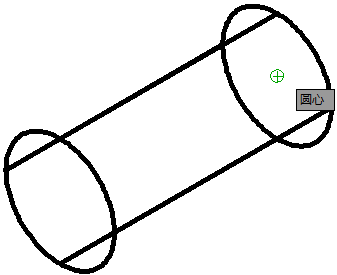
\includegraphics[scale=0.5]{centerselect.png}}\hspace{20pt}
\subfloat[]{\label{fig:beifront}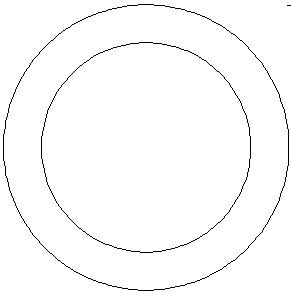
\includegraphics[scale=0.5]{beifront.png}}
\caption{杯块零件主视图绘制}
\end{figure}
\end{procedure}

至此,我们已经完成了杯块零件的主视图绘制,下面对绘图过程的关键点说明如下:
\showremarks

\endinput